%%%%%%%%%%%%%%%%%%%%%%%%%%%%%%%%%%%%%%%%%
% Focus Beamer Presentation
% LaTeX Template
% Version 1.0 (8/8/18)
%
% This template has been downloaded from:
% http://www.LaTeXTemplates.com
%
% Original author:
% Pasquale Africa (https://github.com/elauksap/focus-beamertheme) with modifications by 
% Vel (vel@LaTeXTemplates.com)
%
% Template license:
% GNU GPL v3.0 License
%
% Important note:
% The bibliography/references need to be compiled with bibtex.
%
%%%%%%%%%%%%%%%%%%%%%%%%%%%%%%%%%%%%%%%%%

%----------------------------------------------------------------------------------------
%	PACKAGES AND OTHER DOCUMENT CONFIGURATIONS
%----------------------------------------------------------------------------------------

\documentclass{beamer}

\usetheme{focus} % Use the Focus theme supplied with the template
% Add option [numbering=none] to disable the footer progress bar
% Add option [numbering=fullbar] to show the footer progress bar as always full with a slide count

% Uncomment to enable the ice-blue theme
\definecolor{main}{RGB}{92, 138, 168}
\definecolor{background}{RGB}{240, 247, 255}

%------------------------------------------------
\usepackage[utf8]{inputenc}
\usepackage{booktabs} % Required for better table rules
\usefonttheme{professionalfonts}
\setbeamerfont{bibliography item}{size=\footnotesize}
\setbeamerfont{bibliography entry author}{size=\footnotesize}
\setbeamerfont{bibliography entry title}{size=\footnotesize}
\setbeamerfont{bibliography entry location}{size=\footnotesize}
\setbeamerfont{bibliography entry note}{size=\footnotesize}
%----------------------------------------------------------------------------------------
%	 TITLE SLIDE
%----------------------------------------------------------------------------------------

\title{A Look at Reciprocal \\ Multifactorial Constants}

\subtitle{}

\author{Bhoris Dhanjal}

\titlegraphic{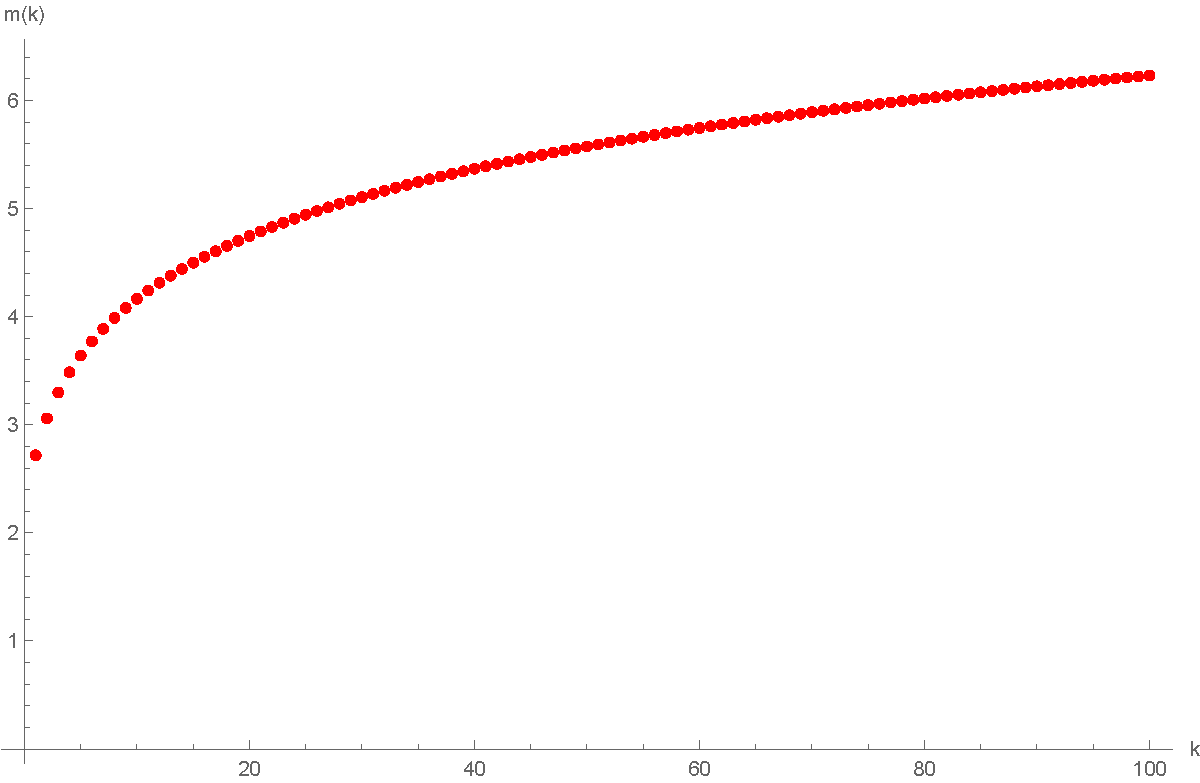
\includegraphics[scale=0.3]{Images/first100rmfc.pdf}} % Optional title page image, comment this line to remove it
\institute{St. Xavier's College\\(Autonomous)}

\date{\today}
%------------------------------------------------

\begin{document}

%------------------------------------------------

\begin{frame}
	\maketitle % Automatically created using the information in the commands above
\end{frame}

%----------------------------------------------------------------------------------------
%	 SECTION 1
%----------------------------------------------------------------------------------------

\section{Section 1: Multifactorials} % Section title slide, unnumbered


\begin{frame}{Definition of a Multifactorial}
We define the multifactorial $n\underbrace{!\ldots!}_{\text{k times}}$ or $n!_{(k)}$ for $n \in \mathbb{N}_0, k \in \mathbb{N}$ by comparing it to the factorial.
\begin{align*}
    n!&=n\cdot(n-1)\cdot(n-2)\cdot(n-3)\dots && \textit{Terminates with 1}
    \intertext{Using steps of larger integer values we get,}
    n!! &=n\cdot(n-2)\cdot(n-4)\cdot(n-6)\dots && \textit{Terminates with 2 or 1}\\
    n!!! &=n\cdot(n-3)\cdot(n-6)\cdot(n-9)\dots && \textit{Terminates with 3, 2 or 1}\\
    & \vdots
\end{align*}\par
\end{frame}

\begin{frame}{Definition of a Multifactorial contd.}
Using this we can alternatively define the multifactorial of any $n>0$ of order $k>0$ as the follows:
\begin{align}
    n!_{(k)}&=\prod_{j=0}^{q}kj+r && \text{where}\ n=kq+r,q\geq 0, \text{and}\ 1\leq r \leq k\\
    &=1 && n=0 \nonumber
\end{align}\par
The above definition is identical to the recursive relation:
\begin{align}
    n!_{(k)} =   \begin{cases}
1 & \text{if $n=0$} \\
n & \text{if $0<n\leq k$} \\   n\left((n-k)!_{(k)}\right) & \text{if $n>k$}   \end{cases}
\end{align}
    
\end{frame}

%------------------------------------------------
\begin{frame}{Reciprocal Multifactorial Series}
    The Reciprocal Multifactorial Series for multifactorial of order $k$ is defined as the follows:
\begin{align}
    m(k)&=\sum_{n=0}^{\infty}\frac{1}{n!_{(k)}}=1+\sum_{r=1}^{k}\sum_{q=0}^{\infty}\frac{1}{(kq+r)\underbrace{!\dots!}_{\text{k times}}}
\end{align}
\end{frame}
%------------------------------------------------
\begin{frame}{Reciprocal Multifactorial Series contd.}
    \begin{columns}
		\column{0.4\textwidth}
			\begin{table}[]
			\tiny
\centering
\begin{tabular}{@{}cc@{}}
\toprule
m(k) & $\sum_{n=0}^{2000}\frac{1}{n!_{(k)}}$  \\ & Rounded to 10 significant digits \\ \midrule
m(1) & 2.718281828 \\
m(2) & 3.059407405 \\
m(3) & 3.298913538 \\
m(4) & 3.485944977 \\
m(5) & 3.640224468 \\
m(6) & 3.771902396 \\
m(7) & 3.886959654 \\
m(8) & 3.989241213 \\
m(9) & 4.081375520 \\
m(10) & 4.165243766 \\ \bottomrule
\end{tabular}
\caption{\small Computed values of first 10 RMFCs \cite{oeis}}
\label{tab:summationvalues}
\end{table}
		
		\column{0.6\textwidth}
			\begin{figure}[!htp]
    \centering
    
\includegraphics[width=\linewidth]{Images/first20partialfractions.png}
    \caption{First 20 partial sums of first 10 Reciprocal Multifactorial Series}
    \label{fig:50partialsums}
\end{figure}
	\end{columns}
\end{frame}
%------------------------------------------------
\section{Section 2: \\Closed Form Formula for RMFCs}
%------------------------------------------------
\begin{frame}{Prerequisites}
    A few prerequisite definitions \cite{gamma} \cite{beta} \cite{incompletegamma}
    \begin{align}
    &\text{Gamma Function } \Gamma (z)=\int_0^{\infty}x^{z-1}e^{-x}dx\text{ for } \text{Re}(z)>0\\
    &\text{Beta Function }  \text{B}(x, y)=\int_0^1 t^{x-1}(1-t)^{y-1} dt \text{ for } \text{Re}(x), \text{Re}(y)>0 \\
    &\text{B}(x,y)=\frac{\Gamma(x)\Gamma(y)}{\Gamma(x+y)}\\
    &\text{Lower incomplete gamma function } \gamma (a, x) = \int_0^x t^{a-1} e^{-t} dt
\end{align}
\end{frame}
%------------------------------------------------
\begin{frame}{Closed Form Formula for RMFCs}
\begin{lemma}
Relation between $k^{th}$ multifactorial and Beta function is given by $$n!_{(k)}=\frac{k^{q+1}q!}{\mathrm{B}\left (\dfrac{r}{k}, q+1\right )}$$
\end{lemma}
\end{frame}
%------------------------------------------------
\begin{frame}{Closed Form Formula for RMFCSs contd.}
\textbf{Proof: }Recall the definition of multifactorial as described in eq. 1.
\begin{align*}
    n\underbrace{!\ldots!}_{\text{k times}}=n!_{(k)}&=\prod_{j=0}^q(kj+r)=k^{q+1}\prod_{j=0}^q\left(j+\frac rk\right)\\
&=k^{q+1}\frac{\Gamma(q+1+\frac{r}{k})}{\Gamma(r/k)}=\frac{k^{q+1}\Gamma(q+1)}{\mathrm{B}\left (\dfrac{r}{k}, q+1\right )} \text{ (from eq. 6)}\\
&=\frac{k^{q+1}q!}{\mathrm{B}\left (\dfrac{r}{k}, q+1\right )} \text{ (since q is a positive integer)}\\
&& \square
\end{align*}
    
\end{frame}
%------------------------------------------------
\begin{frame}{Closed Form Formula for RMFCs contd.}
    \begin{theorem}A closed form formula for Reciprocal Multifactorial Constants is given by the following expression \cite{stackproof}
$$m(k)=1+\frac{e^{1/k}}{k}\sum_{r=1}^{k}k^{r/k}\gamma\left ( \frac{r}{k}, \frac{1}{k} \right )$$
\end{theorem}
\end{frame}
%------------------------------------------------
\begin{frame}{Proof of Closed Form Formula for RMFCs}
    \textbf{Proof: }Recall definition 3.1 for reciprocal multifactorial series.
    \begin{align*}
        m(k)&=\sum_{n=0}^{\infty}\frac{1}{n!_{(k)}}=1+\sum_{r=1}^{k}\sum_{q=0}^{\infty}\frac{1}{(kq+r)\underbrace{!\dots!}_{\text{k times}}}\\
    \intertext{Now, using the lemma we get,}
    &=1+\sum_{r=1}^k\sum_{q=0}^\infty\frac{1}{k^{q+1}q!}\mathrm{B}\left(\frac rk,q+1\right)
    \intertext{Using the integral definition for the Beta function (see 4.1.2) we can say,}
    &=1+\sum_{r=1}^k\sum_{q=0}^\infty\frac{1}{k^{q+1}q!}\int_0^1 t^{r/k-1}(1-t)^q\,dt
    \end{align*}
    
   
\end{frame}
%------------------------------------------------
\begin{frame}{Proof of Closed Form Formula for RMFCs contd.}
     \begin{align*}
    &=1+\frac1k\sum_{r=1}^k\int_0^1 t^{r/k-1}\sum_{q=0}^\infty\frac1{q!}\left(\frac{1-t}{k}\right)^q dt\\
    &=1+\frac1k\sum_{r=1}^k\int_0^1 t^{r/k-1}e^{(1-t)/k}\,dt
    \intertext{Taking $t=kx$ we simplify the function as follows,}
    &=1+\frac1k\sum_{r=1}^k\int_0^{1/k} (kx)^{r/k-1}e^{(1-kx)/k}\,k dx\\
    &=1+\frac{e^{1/k}}k\sum_{r=1}^k k^{r/k}\int_0^{1/k}x^{r/k-1}e^{-x}\,dx
    \end{align*}
\end{frame}
%------------------------------------------------
\begin{frame}{Proof of Closed Form Formula for RMFCs contd.}
    Finally using the definition for incomplete gamma function
            \begin{align*}
    =1+\frac{e^{1/k}}k\sum_{r=1}^k k^{r/k}\gamma \left (\frac{r}{k}, \frac{1}{k} \right)\\
    && \square
    \end{align*}

\end{frame}
%------------------------------------------------
%------------------------------------------------
\begin{frame}{Reciprocal Multifactorial Series contd.}
    \begin{columns}
		\column{0.5\textwidth}
			\begin{figure}[!hbp]
            \centering
              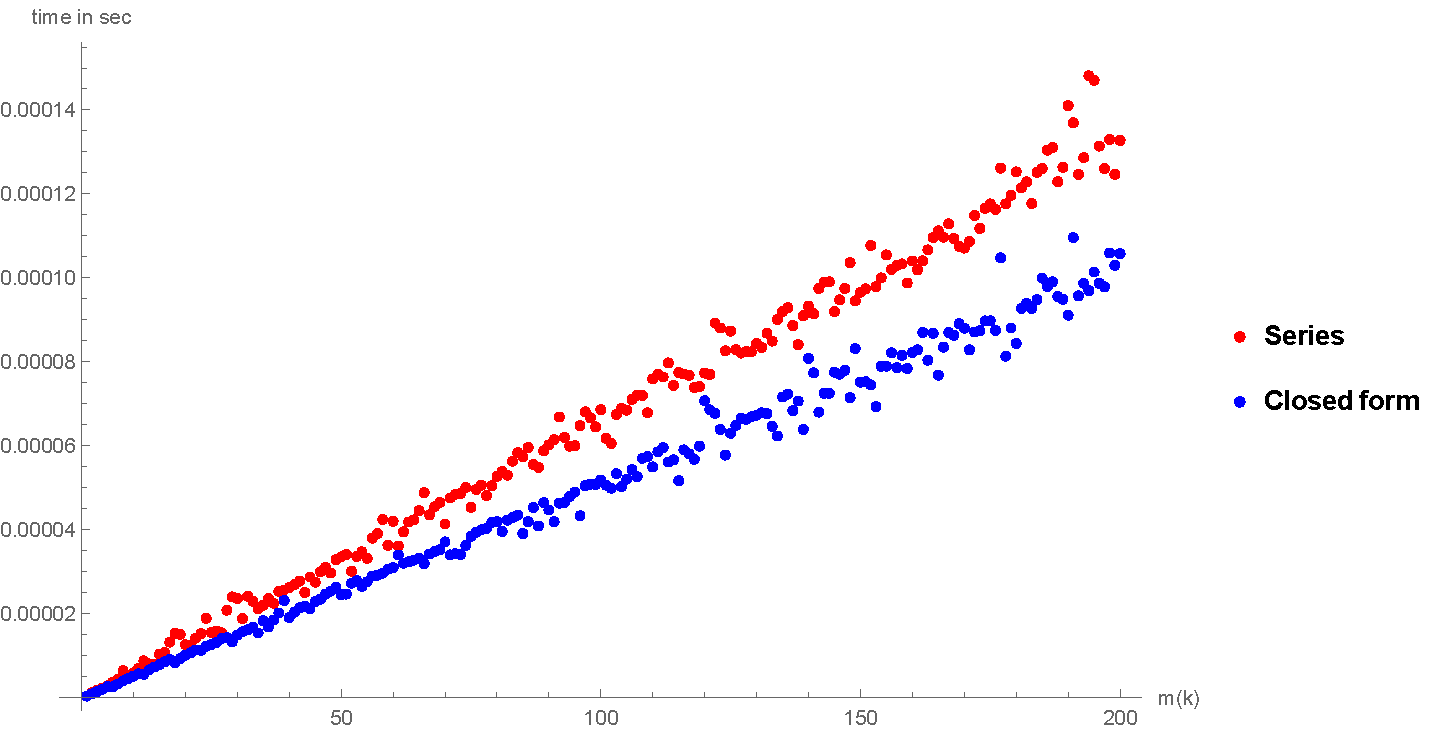
\includegraphics[width=\linewidth]{Images/first200RMFCseriesvsclosedform.pdf}
                \caption{Time taken to compute a list of first k RMFCs (k ranging from 1 to 200) up to 50 digit accuracy.}
              \label{fig:timecompfirst200rmfcs}
            \end{figure}
		\column{0.5\textwidth}
			\begin{figure}[!hbp]
             \centering
             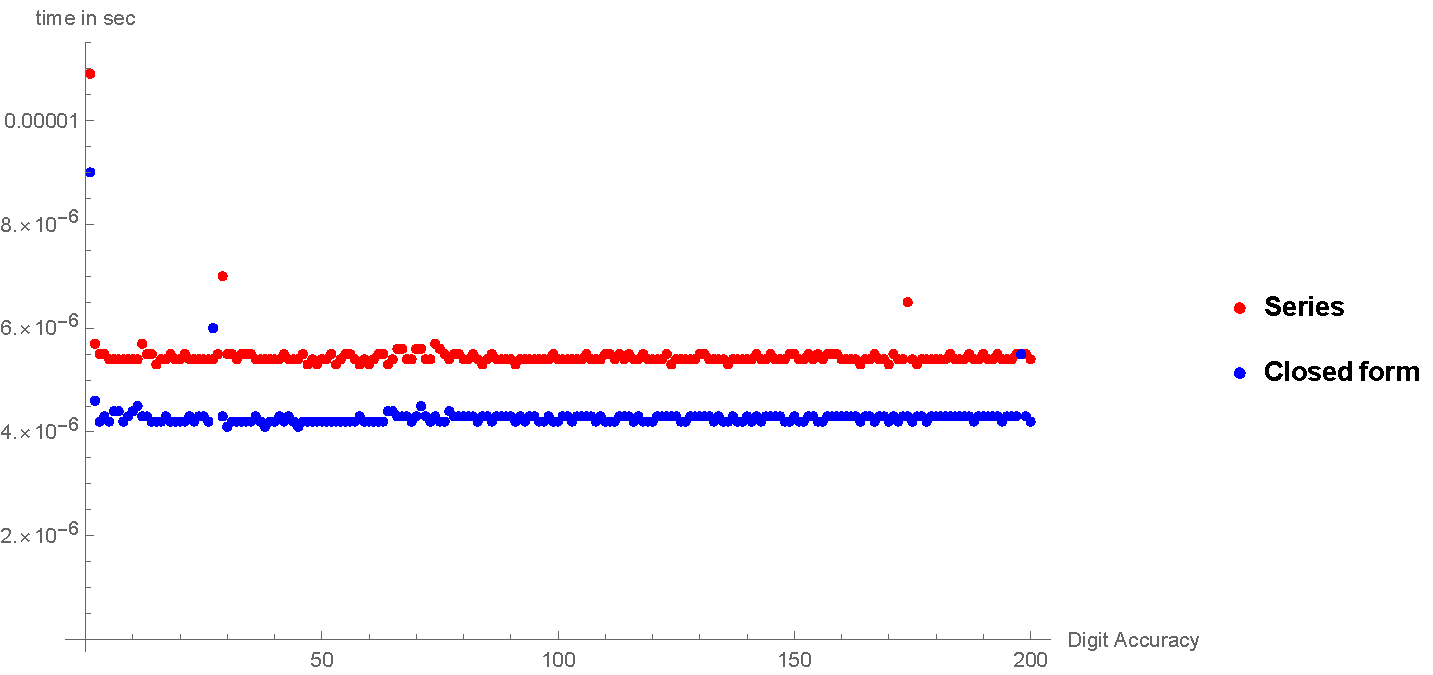
\includegraphics[width=\linewidth]{Images/first200digitsaccuracy.pdf}
             \caption{Time taken to compute first 10 RMFCs with increasing accuracy up to 200 digit accuracy.}
              \label{fig:timecomp10rmfc200digit}
            \end{figure}
	\end{columns}
\end{frame}
%------------------------------------------------
\section{Section 3:\\Asymptotics of Reciprocal \\Multifactorial Series}
%------------------------------------------------
\begin{frame}{Divergent nature of RMFCs for large k}
\begin{theorem}
$\lim_{k\rightarrow \infty} m(k) = 1+H_k$
\end{theorem}
\textbf{Proof: }Continuing from the previous proof, \cite{stackasymptote}
\begin{align*}
m(k)&=1+\frac{e^{1/k}}{k}\sum_{r=1}^k\int_0^1 t^{r/k-1}e^{-t/k}\,dt
    \intertext{Observe that $e^{-t/k}=1-(1-e^{-t/k})$}
    &=1+\frac{e^{1/k}}{k}\sum_{r=1}^k\int_0^1 t^{r/k-1}(1-(1-e^{-t/k}))\,dt
    \intertext{Since, $\int_0^1 t^{r/k-1}\,dt=\frac{k}{r}$, we can further simplify the above expression as}
\end{align*}
\end{frame}
%------------------------------------------------
\begin{frame}{Divergent nature of RMFCs for large k contd.}
\begin{align*}
    &=1+e^{1/k} \left(H_k-\frac{1}{k} \int_0^1 \sum_{r=1}^k t^{r/k}\frac{(1-e^{-t/k})}{t}\,dt \right)\\
    &=1+e^{1/k} \left(H_k-\frac1k\int_0^1\frac{(1-t)(1-e^{-t/k})}{t(t^{-1/k}-1)}\,dt.\right)
    \intertext{Replacing $\frac1k\int_0^1\frac{(1-t)(1-e^{-t/k})}{t(t^{-1/k}-1)}\,dt.$ with $\Delta k$ we get, }
    m(k)&=1+e^{1/k}\left( H_k - \Delta k \right)
    \intertext{Taking the limit as k approaches infinity we get,}
    \lim_{k\rightarrow \infty} m(k)&=\lim_{k\rightarrow \infty} 1+e^{1/k}(H_k - \Delta k)\\
    \lim_{k\rightarrow \infty} m(k)&=1+H_k && \square
\end{align*}
    
\end{frame}
%------------------------------------------------
\begin{frame}{Asymptotic Approximations for RMFCs}
    We will generate asymptotic approximations for RMFCs using the following series, \cite{harmonicwolfram}\cite{expwolfram}\cite{emconstant}
    \begin{align}
    e^{1/k}&=1+\frac{1}{k}+\frac{1}{2 k^2}+O\left (\frac{1}{k^3}\right )\\
    H_k&=\log(k)+\gamma+\frac{1}{2k}-\frac{1}{12k^2}+O\left (\frac{1}{k^4}\right )\\
    \Delta k&=\frac{\log(2)}{k}+\frac{1}{4k^2}\left( -1-\log \frac{9}{4}
    \right) + O\left(\frac{1}{k^3} \right)
\end{align}
\end{frame}
%------------------------------------------------
\begin{frame}{Asymptotic Approximations for RMFCs contd.}
\textbf{Approximation 1:} Using asymptotic series truncated at $1^{st}$ order terms
\begin{align*}
    m(k)&=1+e^{1/k}\left( H_k - \Delta k \right)\\
    m(k) &\sim 1+\left( 1+ \frac{1}{k} \right) \left( \left( \log(k) + \gamma + \frac{1}{2k} \right) - \left( \frac{\log(2)}{k} \right) \right)
\end{align*}
Which can be simplified as the following,
\begin{align}
    m(k) \sim 1+ \frac{(1+k)(1+2 \gamma k - \log (4) +2k \log(k))}{2k^2}
\end{align}
    
\end{frame}
%------------------------------------------------

\begin{frame}{Asymptotic approximations for RMFCs contd.}
\textbf{Approximation 2:} Using asymptotic series truncated at $2^{nd}$ order terms
\begin{equation*}
    \begin{aligned}
    m(k)&=1+e^{1/k}\left( H_k - \Delta k \right)\\
    m(k)& \sim 1+\left(1+\frac{1}{k}+\frac{1}{2 k^2} \right) \left[ \left( \log(k)+\gamma+\frac{1}{2k}-\frac{1}{12k^2} \right) \right.-\\
    &\left. \left( \frac{\log(2)}{k}+\frac{1}{4k^2}\left( -1-\log \frac{9}{4}\right) \right)\right]
\end{aligned}
\end{equation*}
Which can be simplified as the following,
\begin{equation}
    m(k) \sim 1+\frac{(1+2k(1+k)\cdot(1+\log\frac{27}{8}+6k^2 \log k +k(3+6\gamma k-\log 64))}{12k^4}
\end{equation}
    
\end{frame}
%------------------------------------------------
\begin{frame}{Accuracy of asymptotic approximations for RMFCs}
    \begin{columns}\scriptsize
            \column{0.5\textwidth}
            \begin{table}[h!]
\centering
\begin{tabular}{@{}cc@{}}
\toprule
m(k) & \begin{tabular}[c]{@{}c@{}}Absolute error between asymptotic\\ approximation and exact solution\end{tabular} \\ \midrule
$1$ & $3.49539 \cdot 10^{-1}$\\
$10$ & $4.49172 \cdot 10^{-3}$ \\
$10^2$ & $4.76604 \cdot 10^{-5}$ \\
$10^3$ & $4.84353 \cdot 10^{-7}$ \\
$10^4$ & $4.87866 \cdot 10^{-9}$ \\ \bottomrule
\end{tabular}\par
\caption{Comparison between first asymptotic equation and exact solution for a few RMFCs}
\label{tab:asymptoticvsexact1}
\end{table}
            \column{0.5\textwidth}
\begin{table}[h!]
\centering
\begin{tabular}{@{}cc@{}}
\toprule
m(k) & \begin{tabular}[c]{@{}c@{}}Absolute error between asymptotic\\ approximation and exact solution\end{tabular} \\ 
\midrule
$1$ & $6.08426 \cdot 10^{-2}$ \\
$10$ & $7.79859 \cdot 10^{-5}$ \\
$10^2$ & $1.14278 \cdot 10^{-7}$ \\
$10^3$ & $1.29004 \cdot 10^{-10}$ \\
$10^4$ & $1.37156 \cdot 10^{-13}$ \\ \bottomrule
\end{tabular}\par
\caption{Comparison between second asymptotic equation and exact solution for a few RMFCs}
\label{tab:asymptoticvsexact2}
\end{table}
    \end{columns}
\end{frame}
%------------------------------------------------
\section{Section 4:\\Generalized Reciprocal \\Multifactorial Constants
}
%------------------------------------------------
\begin{frame}{Definition of Generalized Reciprocal \\Multifactorial Constants}
    In this section we will discuss the power series reciprocal multifactorial series. For simplicity sake we will refer to these power series as \emph{Generalized Reciprocal Multifactorial Series}.
Which we define as follows,
\begin{align}
    m_x(k)=\sum_{n=0}^\infty \frac{x^n}{n!_{(k)}}=1+\sum_{r=1}^{k}\sum_{q=0}^{\infty}\frac{x^{kq+r}}{(kq+r)\underbrace{!\dots!}_{\text{k times}}}
\end{align}
\par The radius for the above power series can be seen to be infinity for all finite $k$.
\end{frame}
%------------------------------------------------
\begin{frame}{Closed form formula for GRMFCs}
    \begin{theorem}A closed form formula for Generalized Reciprocal Multifactorial Constants is given by the following expression
$$m_x(k)=1+\frac{e^{x^k/k}}{k}\sum_{r=1}^{k}k^{r/k}\gamma\left ( \frac{r}{k}, \frac{x^k}{k} \right )$$
\end{theorem}
\end{frame}
%------------------------------------------------
\begin{frame}{Proof of Closed Form Formula for GRMFCs}
\textbf{Proof: } We continue similarly to the previous theorem,
    \begin{align*}
    m_x(k)&=\sum_{n=0}^{\infty}\frac{x^n}{n!_{(k)}}=1+\sum_{r=1}^{k}\sum_{q=0}^{\infty}\frac{x^{kq+r}}{(kq+r)\underbrace{!\dots!}_{\text{k times}}}\\
    \intertext{Using the lemma we get,}
    &=1+\sum_{r=1}^k\sum_{q=0}^\infty\frac{x^{kq+r}}{k^{q+1}q!}\mathrm{B}\left(\frac rk,q+1\right)
    \intertext{Using the integral definition for the Beta function,}
    &=1+\sum_{r=1}^k\sum_{q=0}^\infty\frac{x^{kq+r}}{k^{q+1}q!}\int_0^1 t^{r/k-1}(1-t)^q\,dt\\
    \end{align*}
\end{frame}
%------------------------------------------------
\begin{frame}{Proof of Closed Form Formula for GRMFCs contd.}

    \begin{align*}
        &=1+\frac1k\sum_{r=1}^k\int_0^1  x^r t^{r/k-1}\sum_{q=0}^\infty\frac{1}{q!}\left(x^k\frac{1-t}{k}\right)^q dt\\
        &=1+\frac1k\sum_{r=1}^k\int_0^1 x^r t^{r/k-1}e^{(x^k-x^k t)/k}\,dt\\
    &=1+\frac{e^{x^k/k}}{k}\sum_{r=1}^k x^r \int_0^1 t^{r/k-1}e^{(-x^k t)/k}\,dt
    \intertext{Let, $u=x^k t/k, dt=k x^{-k} du, t=u k/ x^k$}
    &=1+\frac{e^{x^k/k}}{k}\sum_{r=1}^k x^r  \int_0^{x^k/k} \left (\frac{u k}{x^k} \right)^{r/k-1}e^{-u}k x^{-k}\,du\\
    \end{align*}
\end{frame}
%------------------------------------------------
\begin{frame}{Proof of Closed Form Formula for GRMFCs contd.}
\begin{align*}
&=1+\frac{e^{x^k/k}}{k}\sum_{r=1}^k x^r (k x^{-k}) (k^{r/k-1} x^{k - r}) \int_0^{x^k/k} u^{r/k-1}e^{-u}\,du\\
\intertext{Simplifying we get,}
        &=1+\frac{e^{x^k/k}}{k}\sum_{r=1}^k k^{r/k} \int_0^{x^k/k} u^{r/k-1}e^{-u}\,du\\
    &=1+\frac{e^{x^k/k}}{k}\sum_{r=1}^k k^{r/k} \gamma \left(\frac{r}{k}, \frac{x^k}{k} \right) && \square
\end{align*}
    
\end{frame}
%------------------------------------------------
\begin{frame}{Few computed examples}
\begin{table}[h!]
\centering
\begin{tabular}{@{}cccccc@{}}
\toprule
x$\backslash$k & $1$ & $2$ & $3$ & $4$ & $5$ \\ \midrule
$0.5$ & $1.64872$ & $1.67697$ & $1.68663$ & $1.69039$ & $1.69195$ \\
$1.0$ & $2.71828$ & $3.05941$ & $3.29891$ & $3.48594$ & $3.64022$ \\
$1.5$ & $4.48169$ & $6.42488$ & $9.06146$ & $13.1533$ & $20.2725$ \\
$2.0$ & $7.38906$ & $16.2285$ & $45.7755$ & $219.471$ & $2.85031$ $\cdot 10^3$ \\
$2.5$ & $12.1825$ & $50.9309$ & $589.300$ & $7.02993$ $\cdot 10^4$ & $1.43833$ $\cdot 10^9$ \\ \bottomrule
\end{tabular}
\caption{Few computed values of GRMFCs using the closed form formula.}
\label{tab:GRMFCexamples}
\end{table}
\end{frame}
%------------------------------------------------
\begin{frame}[allowframebreaks]
        \frametitle{References}
        
        \bibliographystyle{unsrt}
    \tiny{\bibliography{example}}
\end{frame}
%------------------------------------------------
\begin{frame}[focus]
    \textbf{\Huge{Thanks for listening}}
\end{frame}
%------------------------------------------------


\end{document}
